\thispagestyle{plain}
\chapter{Analyse der IceCube 2011 Daten S.20}
\section{Ereignis Eigenschaften}
\begin{figure}
\begin{subfigure}{.33\textwidth}
  \centering
  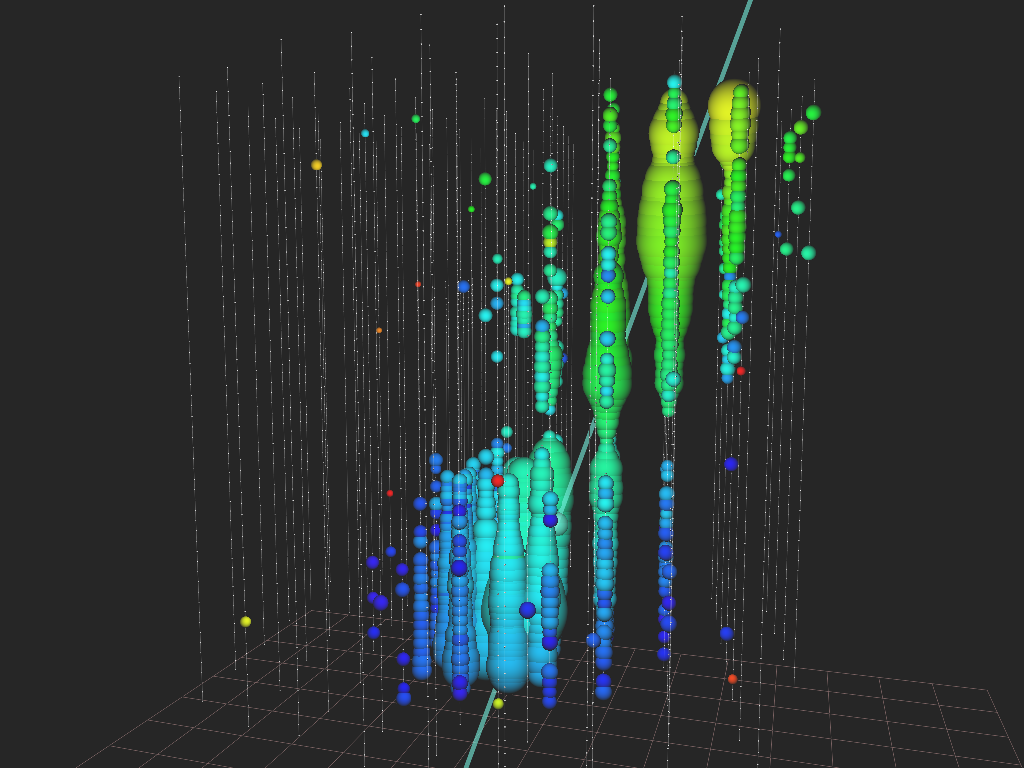
\includegraphics[width=\textwidth]{./Plots/Bundle.png}
  \caption{1a}
  \label{fig:sfig1}
\end{subfigure}%
\begin{subfigure}{.33\textwidth}
  \centering
  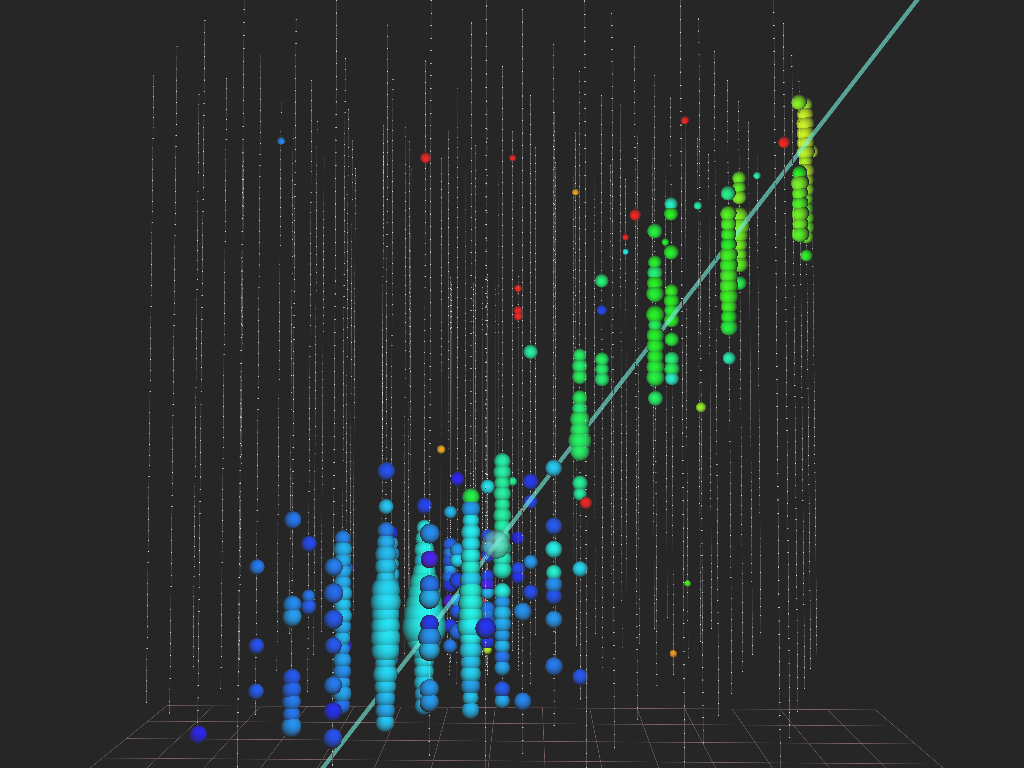
\includegraphics[width=\textwidth]{./Plots/Leading.png}
  \caption{1b}
  \label{fig:sfig2}
\end{subfigure}
\begin{subfigure}{.33\textwidth}
  \centering
  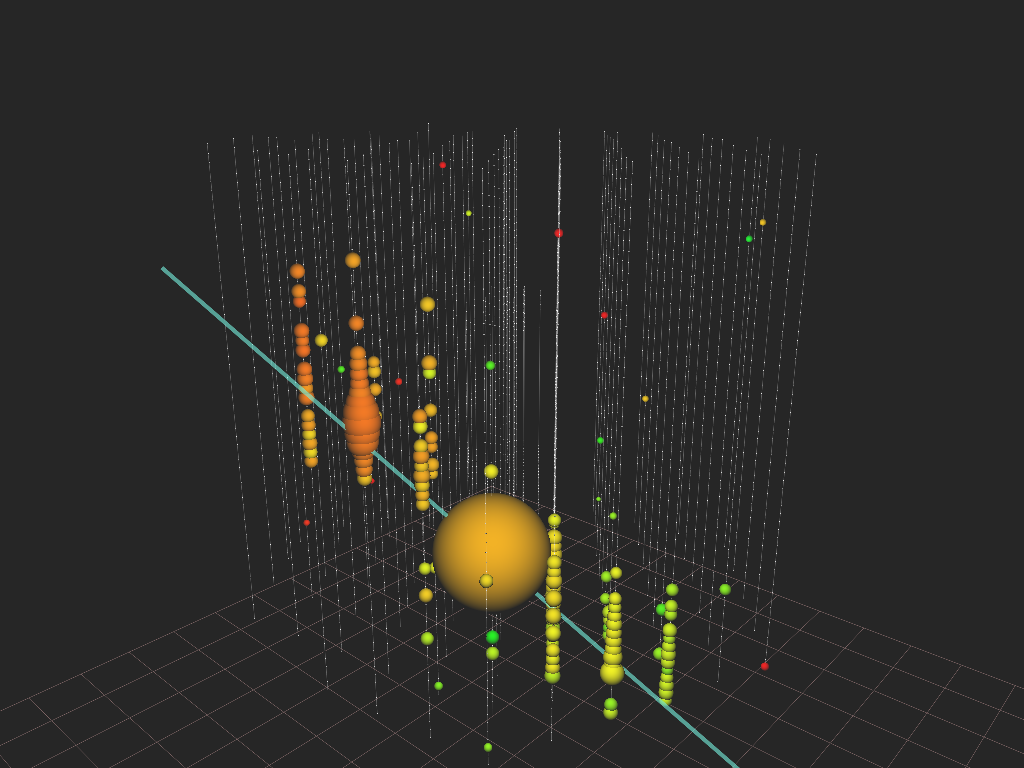
\includegraphics[width=\textwidth]{./Plots/Balloon.png}
  \caption{1b}
  \label{fig:sfig2}
\end{subfigure}
\caption{plots of....}
\label{fig:fig}
\end{figure}
%
\includegraphics[width=\textwidth]{./Plots/dummy.png}
Bei der detektion von Myonen in IceCube treten prinzipiell drei verschiedene Ereignis Typen auf. Diese Ereignisse werden in dieser Arbeit als hochenergetische Myonen (im folgendenen als HE-Myon-Ereignisse bezeichnet), Balloon-Ereignisse und Myon-Bündel-Ereignisse auf. Alle detektierten Ereignisse sind Myon-Bündel-Ereignisse, allerdings ergeben sich die weiteren Klassifikationen durch die Komposition der Myonen in dem Bündel oder anhand der Topologie der detektierten Ereignisse.
\subsection{Myon Bündel}

\subsection{Hochenergetische Myonen}
\subsection{Balloon Ereignisse}
\section{Parameter S.2}
\section{Cuts S.2}
\section{Daten vs. MC S.4}

\newcommand{\nextitem}{\par\hspace*{\labelsep}\textbullet\hspace*{\labelsep}}

\begin{figure}[htbp]
	% minipage mit (Blind-)Text
	\begin{minipage}{0.5\textwidth} 
	SplineMPECharacteristics
	\begin{itemize}
\item track\_hits\_separation\_length
\item track\_hits\_distribution\_smoothness
\item avg\_dom\_dist\_q\_tot\_dom \\
	\end{itemize}

	% \caption{Der Text}
	% \label{Text}
	\end{minipage}
	% Auffüllen des Zwischenraums
	%\hfill
	% minipage mit Grafik
	\begin{minipage}{0.5\textwidth}
	% \textwidth bezieht sich nun auf die Minipage
	
\includegraphics[width=\textwidth]{./Plots/dummy.png}
	\caption{Eine Grafik}
	\label{Bild} 
	\end{minipage}
% \caption{noch eine Caption}
\end{figure}

\begin{table}[!h]
    \label{tab:bsp}
    \begin{tabular}{p{3in}p{3in}}
        \toprule
        HitStatisticsValues.cog\_z              & PoleMuonLlhFitCutsFirstPulseCuts.s\_dir                        \\
HitStatisticsValues.cog\_z\_sigma       & PoleMuonLlhFitFitParams.nmini                                  \\
HitStatisticsValues.z\_max              & SPEFitSingle\_TTFitParams.nmini                                \\
U\_CogRxy                               & U\_DEDXALLDOMS\_L10           \\
U\_DeltaZen                             & U\_QmaxOverQtot \\
%PoleMuonLlhFitCutsFirstPulseCuts 
%	\nextitem s\_dir 
%	\nextitem n\_dir 
%	\nextitem l\_dir              &   SplineMPECharacteristics
%              \nextitem track\_hits\_separation\_length
%              \nextitem track\_hits\_distribution\_smoothness
%              \nextitem avg\_dom\_dist\_q\_tot\_dom \\
U\_SmoothnessE\_ABS                     & SplineMPEDirectHitsA.n\_early\_doms                            \\
SplineMPE.zenith                        & SplineMPEDirectHitsA.n\_early\_strings                         \\
LineFit\_TTParams.lf\_vel               & SplineMPEDirectHitsC.n\_dir\_strings                           \\
LineFit\_TTParams.lf\_vel\_z            & SplineMPEDirectHitsE.dir\_track\_hit\_distribution\_smoothness \\
LineFit\_TTParams.n\_hits               & SplineMPEDirectHitsE.n\_dir\_strings                           \\
MPEFitHighNoiseFitParams.nmini          & SplineMPEFitParams.nmini                                       \\
PoleMuonLlhFitCutsFirstPulseCuts.l\_dir & SplineMPEMuEXDifferential.energy                               \\
PoleMuonLlhFitCutsFirstPulseCuts.n\_dir & SplineMPEMuEXDifferential\_r.value    \\
        \bottomrule
    \end{tabular}        
    \centering
    \caption{Die besten 30 Parameter, welche mit Hilfe des MRMR-Algorithmus ermittelt wurden und zur Trennung der Untergrund- und Signalereignisse genutzt wurden.}
\end{table}


